\subsection{Kociemba's Optimal Solver}
When we look at improving our implementation of Kociemba's optimal solver some different things can be done.
	
%When the \rubik{} is solved from an arbitrary position into H it is not possible to look at it from other angels. 
In the first phase of our implementation of Kociemba's optimal solver we check after every tested move sequence if the \cube{} is in \m{H}.
This \m{H} is with respect to the primary \face{}s (see sub section \ref{sub:theSubgroupH}), but it is also possible for the \rubik{} to be inside \m{H} with respect to the secondary \face{}s or tertiary \face{}s, see figure \ref{}.

\begin{figure}
	\centering
	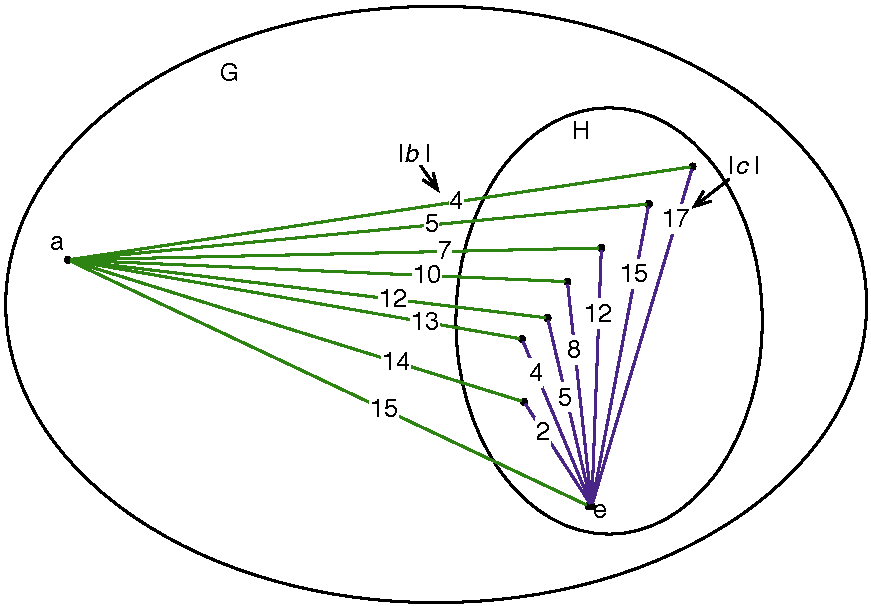
\includegraphics[scale=0.75]{input/pics/kocieambe2.pdf}
	\caption{\myCaption{The lines going from $a$ to a point in $H$ is the move sequence denoted $b$. The lines from points in $H$ to the point $e$ is the move sequence denoted $c$ . The numbers beside the lines are the number of moves. Note that the moves in $c$ is decreasing as the numbers of moves in $b$ is increasing. The line that goes directly from $a$ to $e$ is the shortest move sequence possible. }}
	\label{fig:kociemba2}
\end{figure}

This means that the application will always work with the \face{}s turning the same way (see subsection \ref{sub:cubeFaces}).
To improve this the \rubik{} could be turned around shifting the \face{}s in the application.
This means that instead of testing if the primary \face{} \cubie{}s are orientated correct it would test if the secondary \face{} \cubie{}s are orientated correct. 
The same idea also applies to the tertiary \face{}.
	
To decrease the search time when solving a \rubik{}, every know position of the \rubik{} could be saved in a lookup table.
When a shortest path to that position is found it could be saved.
This would shorthen the time to solve the \rubik{} if the position is already know.
If this is combined with the previous improvement suggestion it could make the search time to get into \m{H} shorter.
Turning of the \face{}s only apply outside \m{H} since it would have a negative effect inside \m{H}. 
	 
The program is built up around one \cube{} object.
As a result of this the computer is only able to use one CPU core to work on that \cube{}.
With some modifications it could be possible make a copy of this \cube{} object.
This will make it possible to work on more than one \cube{} object with the same starting position.
It would be possible to make the application multithreaded in alot of ways.
When the application is working outside \m{H} it is working with \m{S} moves.
Here it is possible to make a new thread for every depth the method searches in.
In the same way it is possible to make a new thread for every search depth inside \m{H}.
But there are still more ways to improve the algorithm with multithreading.
The last way we will mention is when searching in general the moves in \m{S} and \m{A} could be divide and a new thread could be made for these new groups of moves.